\PassOptionsToPackage{unicode}{hyperref}
\documentclass[
  ukrainian,
  14pt
]{extreport}
\usepackage{lmodern}
\usepackage{hyperref}
\makeatletter
\hypersetup{
    colorlinks=true,
    linkcolor=blue,
    filecolor=magenta,
    urlcolor=cyan,
}
\makeatother
\usepackage{amssymb,amsmath,amsthm,url}
\usepackage[margin=2cm]{geometry}
\usepackage{longtable,booktabs}
\usepackage{etoolbox}
\usepackage{titling}
\usepackage{graphicx}
\usepackage{float}
\usepackage[dvipsnames]{xcolor}
\usepackage[ukrainian]{babel}
\usepackage{setspace}
\usepackage{xcolor}
\usepackage{multirow}
\usepackage{comment}
\usepackage{booktabs}
\usepackage{tikz}
\setcounter{secnumdepth}{-1} 
\usepackage{unicode-math}
  \defaultfontfeatures{Scale=MatchLowercase}
  \defaultfontfeatures[\rmfamily]{Ligatures=TeX,Scale=1}
  \setmainfont[]{Times New Roman}
  \setsansfont[]{Arial}
  \setmonofont[]{Consolas}
  \makeatother
\usepackage[labelsep=period]{caption}
\usepackage{subcaption}

\author{}
\title{\Huge Лабораторна робота №4 \\\Large Дослідження ВАХ транзисторів}
\date{}
             
\begin{document}
\begin{titlepage} 
	\newcommand{\HRule}{\rule{\linewidth}{0.5mm}} 
	
	\center 
	
	\textsc{\Large МІНІСТЕРСТВО ОСВІТИ І НАУКИ УКРАЇНИ\\ \Large КИЇВСЬКИЙ НАЦІОНАЛЬНИЙ УНІВЕРСИТЕТ ІМЕНІ ТАРАСА ШЕВЧЕНКА}\\[1.5cm] 

	
	\HRule\\[0.4cm]
	
	{\huge \bfseries  Лабораторна робота №4 \\\Large \bfseries Дослідження ВАХ транзисторів
    }\\[0.4cm]
	
	\HRule\\[1.5cm]

	
	

	{\large\textit{Автор}}\\
	\large Столяров Андрій Дмитрович, \\\large група 5-А, Фізичний Факультет 
	
	
	\vfill\vfill\vfill 
	\vfill
	{\normalsize Київ, \today} 
\end{titlepage}
\tableofcontents
\clearpage
\section{Вступ}
Ця лабораторна робота присвячена вивченню вольт-амперних
характеристик транзисторів – керованих нелінійних елементів, на основі
яких можна створювати підсилювачі електричних сигналів.

\subsection{Мета}
дослідити вихідні характеристики транзисторів різних типів.

\subsection{Методи дослідження}
\begin{enumerate}
    \item одержання зображення ВАХ транзисторів на екрані двоканального
    осцилографа, що працює в режимі характериографа,
    \item побудова сімейства ВАХ шляхом вимірювання певної кількості
    значень сили струму $І_{\text{к}}$, що відповідають певним значенням напруги $U_{\text{ке}}$
    (для певної сили струму бази $І_{\text{б}}$ або напруги $U_{\text{бе}}$) для біполярного
    транзистора та певної кількості значень сили струму стоку $І_{\text{с}}$, що
    відповідають певним значенням напруги $U_{\text{св}}$ (для певних значень напруги
    між затвором і витоком $U_{\text{зв}}$) для польового транзистора, подання
    результатів вимірів у вигляді графіків.
\end{enumerate}

\section{Теоретичні відомості}
\textbf{Біполярний транзистор} – це напівпровідниковий прилад з двома p-n–переходами, що взаємодіють між собою, та трьома виводами,
підсилювальні властивості якого зумовлені явищами інжекції (введення) та
екстракції (вилучення) неосновних носіїв заряду.
\textbf{Вихідна вольт-амперна характеристика (ВАХ) біполярного
транзистора} – це залежність сили струму колектора $І_{\text{к}}$ від напруги між
колектором та емітером Uке при певному значенні струму бази $І_{\text{б}}$, (або
напруги між базою та емітером $U_{\text{бе}}$) в схемі зі спільним емітером.
\textbf{Польовий (уніполярний) транзистор} – це напівпровідниковий прилад,
підсилювальні властивості якого зумовлені струмом основних носіїв, що
течуть по провідному каналу, провідність якого керується зовнішнім
електричним полем.
\textbf{Польовий транзистор з керувальним електродом} – це польовий
транзистор, керування струмом основних носіїв у якому здійснюється за
допомогою p-n–переходу, зміщеного у зворотному напрямі.
\textbf{Вихідна вольт}-амперна характеристика (ВАХ) польового
транзистора – це залежність сили струму стоку $І_{\text{с}}$ від напруги між стоком
та витоком $U_{\text{св}}$ при певному значенні напруги між затвором та витоком
$U_{\text{зв}}$.
Біполярний транзистор являє собою сукупність двох p-n–переходів,
складених з двох p-областей і однієї n-області (структура типу p-n-p) або з
двох n-областей і однієї p-області (структура типу n-p-n). Одна з крайніх
областей носить назву емітера, а інша – колектора, середню область
називають базою. База-емітерний (або просто емітерний) p-n-перехід
включають у прямому напрямку, а база-колекторний (або просто
колекторний) p-n-перехід – у зворотному
Принцип роботи польових транзисторів простіший за принцип дії
біполярних транзисторів. Польовий транзистор являє собою
триелектродний прилад, в якому струм створюють основні носії заряду під
дією повздовжнього електричного поля, а керування величиною цього
струму здійснюється поперечним електричним полем, що створюється
напругою, прикладеною до керувального електрода.

\section{Хід Роботи}
\subsection{Біполярний транзистор}
\begin{figure}[H]
    \centering
    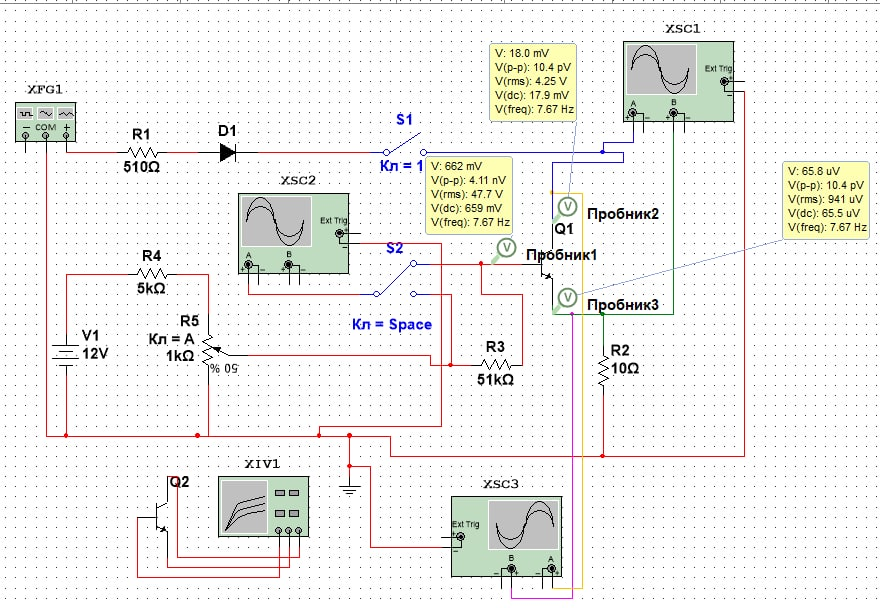
\includegraphics[width=.7\textwidth]{imgs/b-1.png}
    \caption{Схема}
\end{figure}
Схема наведена у файлі \textbf{\underline{ВАХ біполярного транзистора.ms14}}.
Переключаючи \textbf{S1} можна вмикати, або вимикати генератор змінного струму. \textbf{S2} відповідає за вмикання додаткового опору і вимірювання напруги безпосередньо на базі транзистора. Підкюлчивши характериограф, можемо побачити ВАХ біполярного транзистора.
\begin{figure}[H]
    \centering
    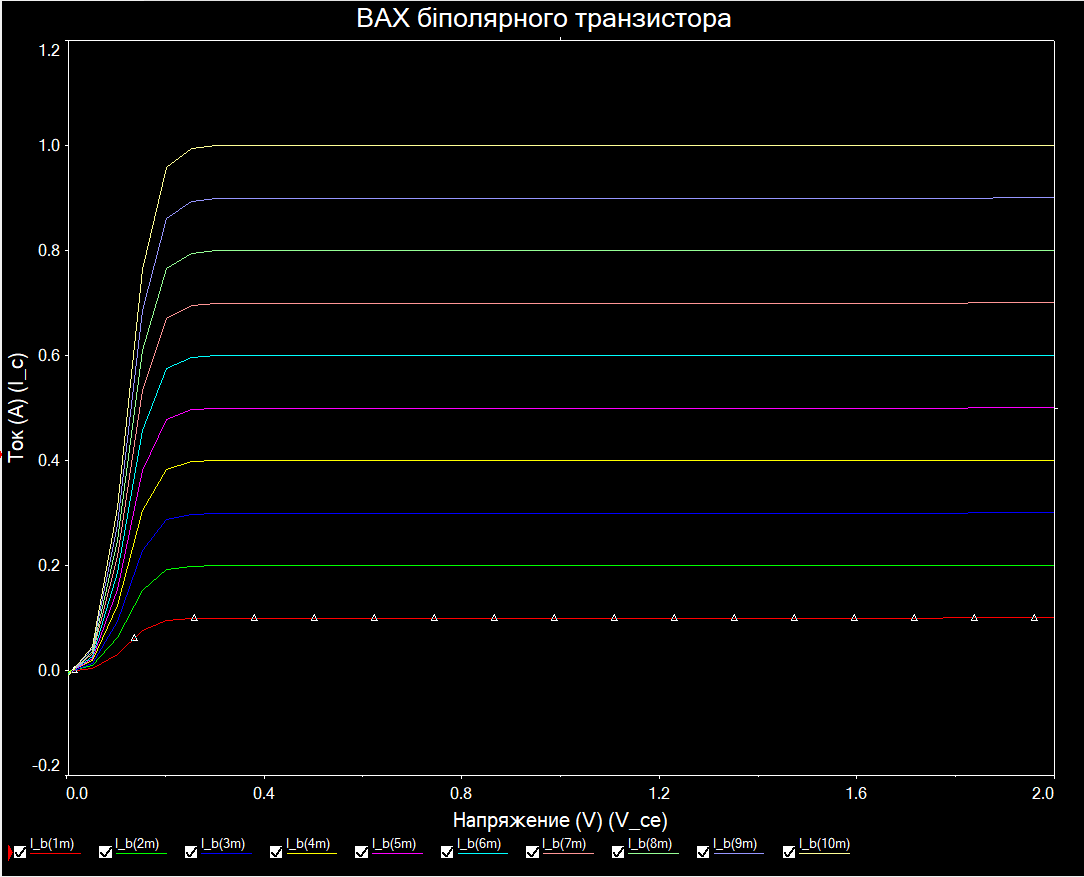
\includegraphics[width=.7\textwidth]{imgs/b-5.png}
    \caption{ВАХ біполярного транзистора}
\end{figure}
\subsection{Польовий транзистор}
\begin{figure}[H]
    \centering
    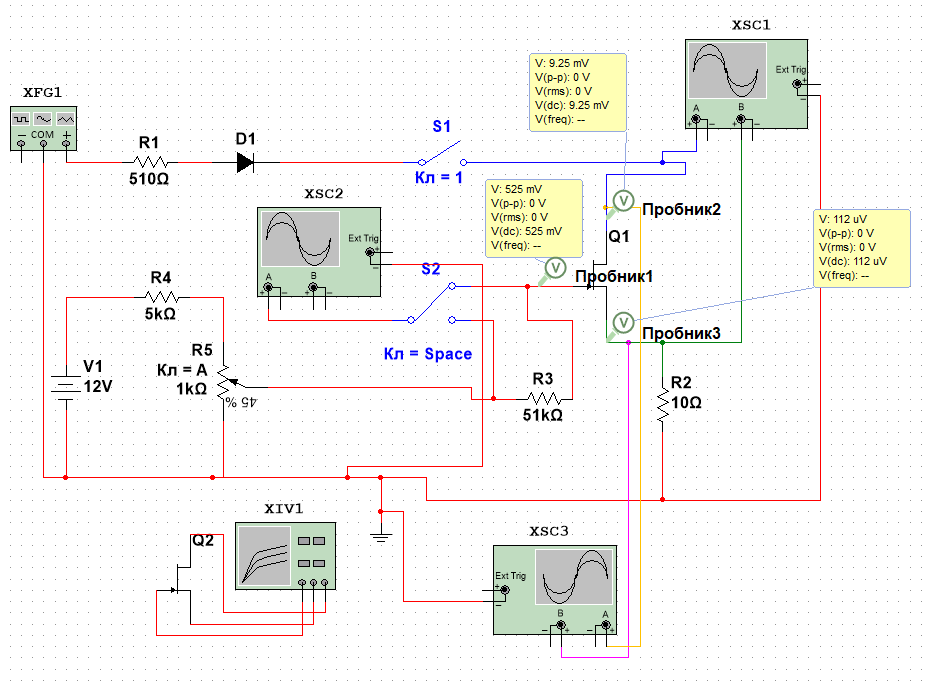
\includegraphics[width=.7\textwidth]{imgs/p-1.png}
    \caption{Схема}
\end{figure}
Схема наведена у файлі \textbf{\underline{ВАХ польового транзистора.ms14}}.
Переключаючи \textbf{S1} можна вмикати, або вимикати генератор змінного струму. \textbf{S2} відповідає за вмикання додаткового опору і вимірювання напруги безпосередньо на базі транзистора. Підкюлчивши характериограф, можемо побачити ВАХ біполярного транзистора.
\begin{figure}[H]
    \centering
    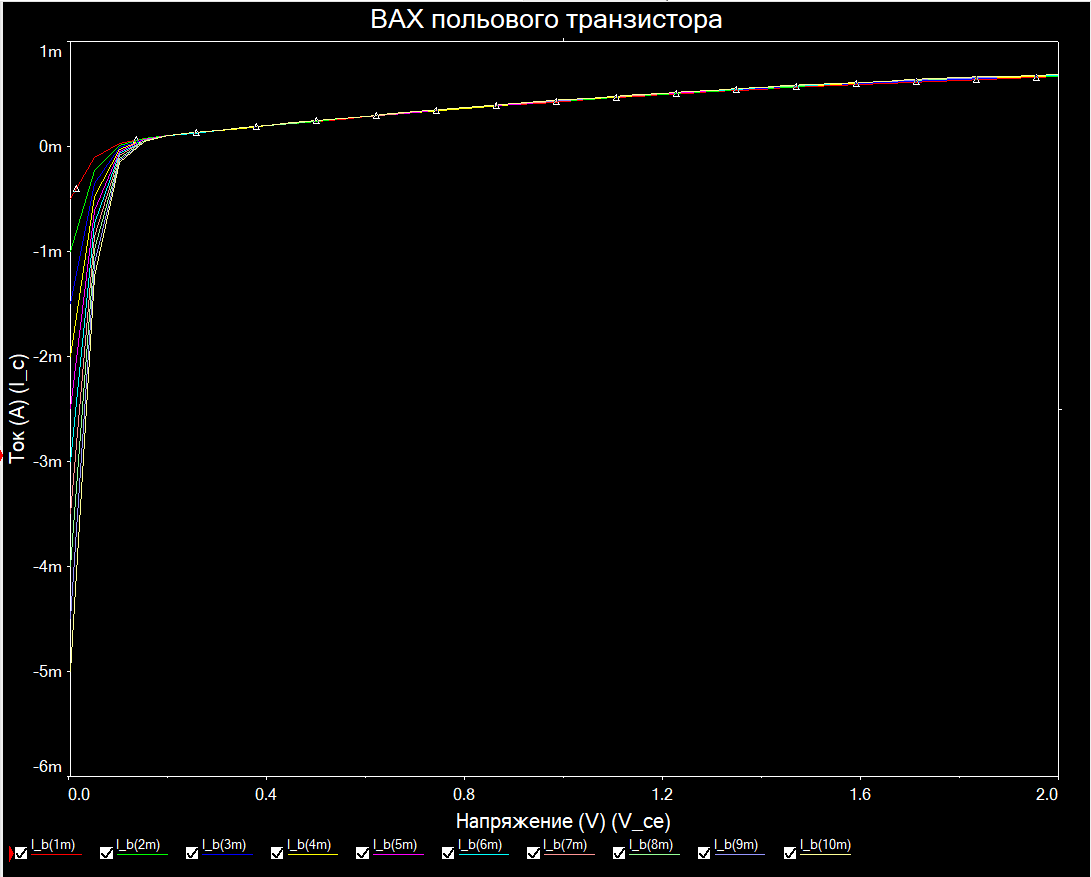
\includegraphics[width=.7\textwidth]{imgs/p-5.png}
    \caption{ВАХ польового транзистора}
\end{figure}


\section{Висновок}
В цій роботі ми отримали графіки напруги на базі транзистора від часу, а
також графіки напруги на еміторі транзистора від напруги на базі.
Дослідження було виконане для 2 типів транзисторів: польового та
біполярного.
Наші графіки вийшли подібні, при різних значеннях на потенціометрі, що і
очікувалося при виконанні лабораторної. 

Робота виконувалась у програмі \textbf{Multisim14}.
\end{document}